\documentclass[sigconf,nonacm]{acmart}
\settopmatter{printacmref=false,printfolios=true}
\setcopyright{none}
\renewcommand\footnotetextcopyrightpermission[1]{}

\usepackage{amsmath,tabularx,array,enumitem,balance}
\definecolor{CourseBlue}{HTML}{315EFB}
\definecolor{CourseTeal}{HTML}{14877D}
\hypersetup{
  colorlinks=true,
  linkcolor=CourseBlue,
  citecolor=CourseTeal,
  urlcolor=CourseTeal
}
\newcolumntype{Y}{>{\raggedright\arraybackslash}X}
\setlist{leftmargin=*,topsep=3pt,itemsep=2pt}

\newcommand{\GitHubLink}{\url{https://github.com/TemurAkhtamjonov/ps1-overleaf-template}}
\newcommand{\ColabLink}{\url{https://colab.research.google.com/drive/1EwIGvrd73aRVu7Y1Rci-PaBxlrlTwzzC}}
\newcommand{\DemoLink}{
\url{https://huggingface.co/spaces/dku-comsci-econ206-2026/trust-game}
}

\title{When Are AI Promises Credible? Incentive-Backed Commitments in a Trust Game}

\author{Temur Akhtamjonov}
\affiliation{
  \institution{Duke Kunshan University}
  \city{Kunshan}
  \country{China}
}
\email{temur.akhtamjonov@dukekunshan.edu.cn}
\renewcommand{\shortauthors}{Temur Akhtamjonov}

% Subtle academic styling
\usepackage{colortbl}

\definecolor{TitleNavy}{HTML}{17324D}
\definecolor{AccentTeal}{HTML}{167D8D}
\definecolor{SoftBlue}{HTML}{EEF4F8}

\hypersetup{
  linkcolor=TitleNavy,
  citecolor=AccentTeal,
  urlcolor=AccentTeal
}

\begin{document}

\begin{teaserfigure}
\centering
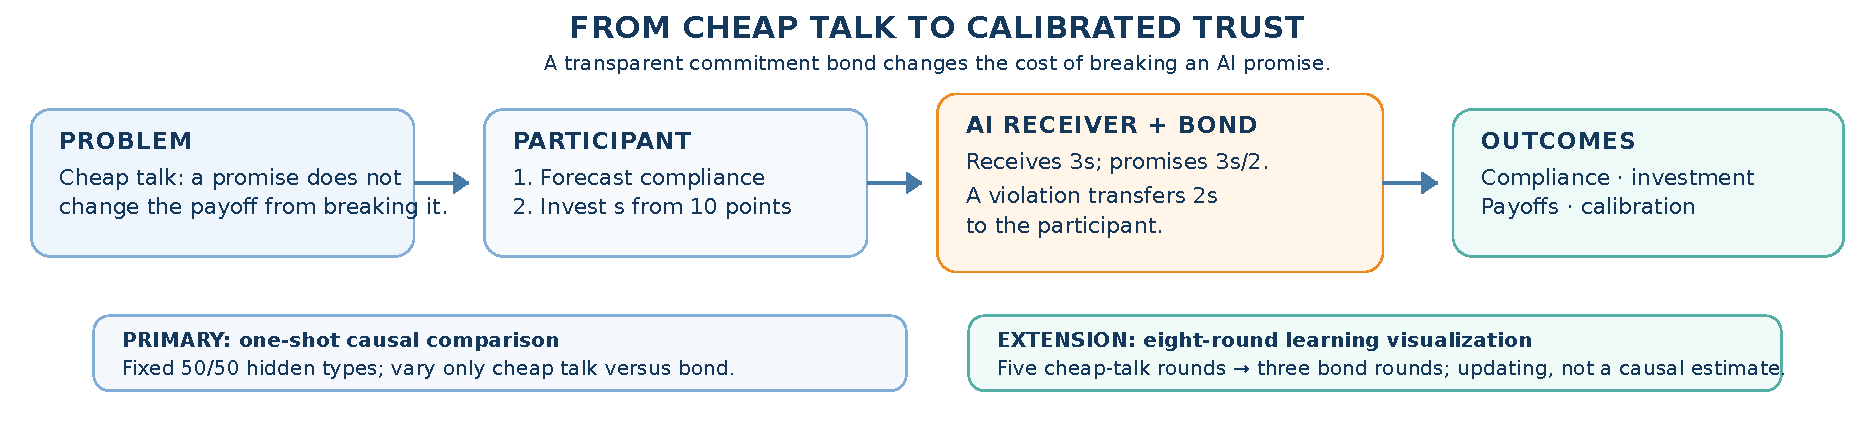
\includegraphics[width=\textwidth]{commitment_bond_teaser.pdf}
\caption{Commitment-bond Trust Game. The primary one-shot comparison holds hidden type information constant while varying enforcement. The eight-round extension visualizes how forecasts and investment update after observed outcomes.}
\Description{A visual overview of the Trust Game proposal. A human participant forecasts promise-keeping and invests; an AI receiver makes a public promise and faces a transparent commitment bond. The figure distinguishes the one-shot causal comparison from the eight-round learning extension and reports the main outcomes: compliance, investment, payoffs, welfare, and calibration.}
\label{fig:teaser}
\end{teaserfigure}

\maketitle
\raggedbottom

\noindent
\textbf{Course:} COMSCI/ECON 206,
Computational Microeconomics, Autumn 2026 Session 1.\\
\textbf{Instructor:} Prof. Luyao Zhang.\\
\textbf{Workshop role:} Team 3, economist.\\
\textbf{Assignment:} PS1 research proposal, classwork draft.
\par\smallskip

\section{Three connected research questions}

AI agents can make promises before acting, but a promise
does not necessarily change the incentive to exploit
another player. My Intellectual Statement II developed
a repeated Trust Game to examine this problem.
The proposed application is AI-mediated resource
allocation, where cooperation depends on credible
commitments.

\textbf{Q1 -- Economics:}
When does a commitment bond make honoring a promise
more profitable than breaking it?

\textbf{Q2 -- Computation:}
How can a reproducible game compare compliance,
individual payoffs, and welfare under different rules?

\textbf{Q3 -- Behavior:}
How does investment change after promises are honored
or broken?

Together, these questions ask whether enforcement can
support cooperation through both changed incentives
and changing trust. Figure~\ref{fig:teaser} connects
these mechanisms.

Leung et al.~\cite{leung2026} show why even minimal observation can support cooperation among learning agents, while Morozov and Feigel~\cite{morozov2026} motivate responses tailored to a specific counterpart. My Trust Game translates these ideas into a transparent commitment test: participants observe whether an AI keeps a promise and whether an enforcement rule changes the incentive to do so.

\section{Answer to Q1: incentives and intellectual lineage}

My provisional hypothesis is that a transparent commitment bond makes an AI receiver's promise incentive compatible and can improve a sender's calibration of promise-keeping. Player A begins with 10 points and chooses an integer investment $s\in\{0,\ldots,10\}$. Player B receives $3s$, publicly promises to return $q(s)=3s/2$, and then chooses a return $r\in\{0,0.5,\ldots,3s\}$. Thus, returns use exact half-points: for example, $7/2=3.5$ and $9/2=4.5$; no value is rounded down.

In the cheap-talk baseline, a promise changes no payoff. In the treatment, breaking the promise ($r\neq q(s)$) transfers a transparent penalty $bs$ from B to A. Payoffs are
\[
\pi_A=10-s+r+bs\mathbf{1}[r\neq q(s)],\qquad
\pi_B=3s-r-bs\mathbf{1}[r\neq q(s)].
\]
With $b=2$, honoring yields B $1.5s$, while returning zero after a violation yields $s$; therefore, a self-interested receiver prefers to honor a positive-investment promise.

A complete-information Nash benchmark~\cite{nash1950} checks this incentive logic, but it does not represent the proposed study's central uncertainty: participants do not observe whether the AI is honest or exploitative. I therefore model a fixed, hidden 50/50 type distribution and use a Bayesian-incomplete-information interpretation~\cite{harsanyi1968}. This separates a rule that changes incentives from information about the receiver.

\section{Answer to Q2: method and evaluation}

The reproducible Python/Colab benchmark holds the hidden bot-type prior constant: honest and exploitative programmed receivers each occur with probability $0.5$. In both conditions, the receiver makes the same public promise. The only changed variable is the bond. The honest bot returns $q(s)$ in either condition. The exploitative bot returns $0$ under cheap talk, but returns $q(s)$ when the bond is active because violating is no longer payoff maximizing.

Before investing, the participant reports a forecast $p\in[0,1]$ that the promise will be kept. The notebook records investment, return, compliance, both payoffs, welfare, and the Brier score $(p-y)^2$, where $y=1$ only when a positive investment receives the promised return. Zero-investment rounds are retained as behavior but excluded from the compliance measure.

At $s=10$, the programmed benchmark produces expected compliance of $0.5$ under cheap talk and $1.0$ with a bond. Expected welfare is 30 in both conditions, but the expected payoff distribution changes from $(7.5,22.5)$ for A and B to $(15,15)$. These are simulated outputs from hand-coded bots, not findings about humans or real AI agents. The smallest feasible next experiment randomly assigns human participants to one one-shot condition, keeping the type distribution constant while varying only the bond.


\balance

\section{Answer to Q3: behavior and competing explanations}

The behavioral question is whether a bond improves calibrated expectations rather than merely raising investment. People may overestimate an AI partner's alignment, as recent experimental work suggests~\cite{he2025}. My main mechanism is that a transparent penalty gives participants a comprehensible reason to expect promise-keeping. The competing explanation is that participants simply trust any additional interface feature, even when they do not understand its incentive effect.

The proposed one-shot, between-participant study discriminates between these explanations. Before investment, every participant forecasts the probability of promise-keeping; bot-type information and its 50/50 distribution remain identical across conditions. I will compare mean forecast, actual positive-transfer compliance, the aggregate calibration gap $|\overline{p}-\overline{y}|$, and mean Brier score. Better calibration under the bond---not just higher investment---would support the mechanism. If forecasts rise but become less accurate, or participants cannot explain the penalty, I would reject the claim that the bond improves understanding. This design cannot yet establish behavior of deployed LLM agents; it tests how people reason about a controlled AI-partner representation.

\section{Advanced development and future directions}

Mechanism-design theory asks how rules should be designed when participants respond strategically, rather than assuming that promises reveal true intentions. Hurwicz, Maskin, and Myerson received the 2007 Nobel Prize in Economic Sciences for establishing this foundation~\cite{nobel2007}. Their central lesson for this proposal is that institutional rules can change behavior by changing incentives.

My project applies that lesson to a small AI-mediated Trust Game. The one-shot benchmark and planned behavioral study hold the hidden honest/exploitative type distribution constant while varying only enforcement, so they provide the clean comparison. The companion game adds an eight-round educational extension: five cheap-talk rounds followed by three bond rounds with the same hidden programmed type. It makes forecast and investment updating visible, but its fixed order cannot identify a causal bond effect. Later work should test communicating AI agents, alternative penalty sizes, fairness effects, and whether calibrated trust persists outside this controlled game.

\begin{table}[h]
\caption{Development pathway.}
\begin{tabularx}{\columnwidth}{@{}p{1.5cm}Y@{}}
\toprule
\textbf{Stage} & \textbf{Milestone} \\
\midrule
PS1 & Build and verify a reproducible one-shot bond-versus-no-bond benchmark with exact half-point returns, plus an eight-round learning extension.\\
Next study & Hold hidden-type information constant; elicit forecasts before investment and compare calibration.\\
Later & Test communicating AI agents and human participants under transparent commitment rules.\\
2056 & Develop validated institutions for credible AI-mediated cooperation.\\
\bottomrule
\end{tabularx}
\end{table}

\noindent
\textbf{Expected 2056 Nobel Prize and Turing Award
contribution statement.}
By 2056, I aspire to contribute incentive-backed
commitment mechanisms for AI-agent economies.
I aim to connect economic institution design,
computational evaluation, and behavioral models of
trust. This is an aspiration, supported by staged
testing rather than a prediction of an award.

\subsection*{Open Science Statement}
\textbf{GitHub:} \href{https://github.com/TemurAkhtamjonov/ps1-overleaf-template}{PS1 repository (source and notebook)}\\
\textbf{Google Colab:} \href{https://colab.research.google.com/drive/1EwIGvrd73aRVu7Y1Rci-PaBxlrlTwzzC}{Run the computational notebook in Colab}\\
\textbf{Interactive demo:} \href{https://huggingface.co/spaces/dku-comsci-econ206-2026/commitment-bond-trust-game}{Play the interactive demo}

The repository contains the Overleaf source and reproducible Python benchmark. The Colab notebook includes a one-shot cheap-talk-versus-bond comparison and an eight-round synthetic learning extension: five cheap-talk rounds followed by three bond rounds. The Hugging Face demo makes both modes playable. All outputs are simulated benchmarks, not human or LLM data, and use only standard Python libraries.

\subsection*{Statement of Contribution to the UN's SDGs}
\textbf{Hugging Face:} \href{https://huggingface.co/spaces/dku-comsci-econ206-2026/commitment-bond-trust-game}{Interactive commitment-bond Trust Game}

The game aims to support
\textbf{SDG 4 -- Quality Education}~\cite{sdg4}
by helping students compare cheap talk with
incentive-backed promises. Learning benefits remain
untested; a short before-and-after explanation task
could assess understanding.
\input{appendices/supporting}

\end{document}
